\documentclass[../TDE8_filtrage.tex]{subfiles}%

\begin{document}
\section[s]"3"{Filtre de \textsc{Butterworth} d'ordre 3}
\enonce{%
	On veut réaliser un filtre de \textsc{Butterworth} d'ordre 3, dont le module $H$
	de sa fonction de transfert harmonique en tension $\Hu$ s'exprime~:
	\[H = \abs{\Hu} = \sqrt{\frac{1}{1+\left(\dfrac{\w}{\w_0}\right)^6}} =
		\sqrt{\frac{1}{1+x^6}}
		\qavec
		x = \frac{\w}{\w_0}
	\]
}

\QR{%
	Montrer qu'une fonction de transfert $\Hu = \DS \frac{1}{1+2\jx +
			2(\jx)^2 + (\jx)^3}$ correspond bien à un filtre de
	\textsc{Butterworth} d'ordre 3.
}{%
	Il suffit pour cette question de développer les puissances sur les
	$\jj$, de calculer le module et de développer~:
	\begin{gather*}
		\Hu = \left( 1 + 2\jx - 2x^2 -\jx^3 \right)^{-1}
		\Lra
		\abs{\Hu}
		= \left( (1-2x^2)^2 + (2x - x^3)^2 \right)^{-1/2}\\
		\Lra
		\abs{\Hu}
		= \left( 1-\bcancel{4x^2} + \cancel{4x^4}
		+ \bcancel{4x^2} - \cancel{4x^4} + x^6 \right)^{-1/2}
		= \left( 1+x^6 \right)^{-1/2}
	\end{gather*}
	ce qui correspond bien à un filtre de \textsc{Butterworth} d'ordre 3.
}

\QR{%
	Étudier et représenter le diagramme de \textsc{Bode} asymptotique en
	amplitude de cette fonction de transfert.
}{%
	~

	\vspace{-24pt}
	\begin{minipage}{0.48\linewidth}
		Pour étudier le diagramme de \textsc{Bode} asymptotique, on définit
		d'abord le gain en décibels~: $G_{\dB} = 20\log(\abs{\Hu}) =
			20\log(\left( 1+x^6 \right)^{-1/2}) = -10\log(1+x^6)$. Ensuite, on
		étudie son comportement asymptotique pour $x \ll 1$ et $x \gg 1$~:
		on trouve
		\begin{gather*}
			\boxed{G_{\dB} \underset{x \ll 1}{\sim} 0}
			\qet
			\boxed{G_{\dB} \underset{x \gg 1}{\sim} -60\log(x)}
		\end{gather*}
		d'où le diagramme de \textsc{Bode} asymptotique ci-contre. Par
		rapport à de l'ordre 1 (\SI{-20}{dB/décade}) ou de l'ordre 2
		(\SI{-40}{dB/décade}), l'atténuation des hautes fréquences est
		encore plus prononcé~: une fréquence 10 fois supérieure à $f_0$
		serait atténuée d'un facteur 1000 au lieu d'un facteur 10.
	\end{minipage}
	\hfill
	\begin{minipage}{0.48\linewidth}
		\begin{center}
			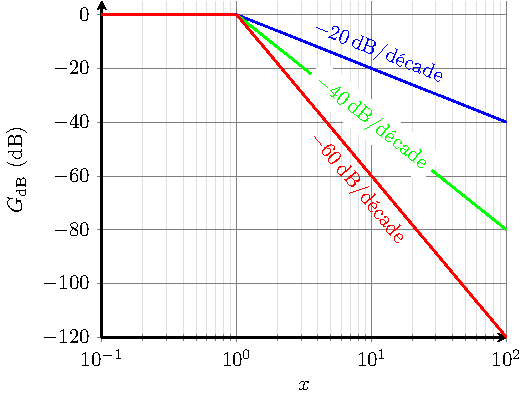
\includegraphics[width=\linewidth]{butterworth_bode-gain}
		\end{center}
	\end{minipage}
}

\QR{%
	On considère le quadripôle ci-dessous~:
	\begin{center}
		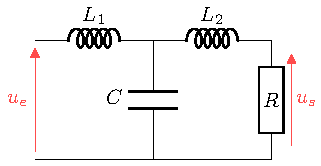
\includegraphics[width=0.5\linewidth]{butterworth_filtre-plain}
	\end{center}
	Calculer en fonction de $R$ et $\w_0$, les valeurs de $L_1$, $L_2$ et
	$C$ pour que ce filtre soit un filtre de \textsc{Butterworth} d'ordre 3.
}{%
	Ici encore, on utilise deux ponts diviseurs de tension successifs~: on
	calcule $u_s$ en fonction de $u_{AB}$, puis $u_{AB}$ en fonction de
	$u_e$ après avoir déterminé l'impédance équivalente de l'ensemble des
	dipôles de droite.
	\begin{center}
		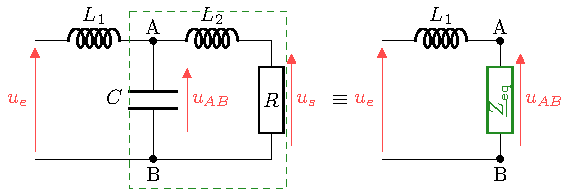
\includegraphics[width=0.8\linewidth]{butterworth_equiv}
	\end{center}
	On aura donc en premier lieu
	\begin{gather*}
		\Uu_s = \frac{\Zu_R}{\Zu_R + \Zu_{L_2}}\Uu_{AB}
		\Lra
		\boxed{\Uu_s = \frac{R}{R+\jj L_2\w}\Uu_{AB}}
	\end{gather*}
	Et ensuite, on aura
	\begin{gather*}
		\Uu_{AB} = \frac{\Zu\ind{eq}}{\Zu\ind{eq} + \Zu_{L_1}}\Uu_e
		\Lra
		\boxed{\Uu_{AB} = \frac{1}{1+\Zu_{L_1}\Yu\ind{eq}}\Uu_e}
	\end{gather*}
	On calcule alors $\Yu\ind{eq}$ de l'association en parallèle de $C$ et
	$L_2$ en série avec $R$~:
	\begin{gather*}
		Z_{L_2+R} = \jj L_2\w + R\\
		\Yu\ind{eq} = \Yu_C + \Yu_{L_2+R}
		\Lra
		\Yu\ind{eq} = \jcw + \frac{1}{\jj L_2\w + R}
		\Lra
		\Yu\ind{eq} = \frac{\jcw (\jj L_2\w + R)+1}{\jj L_2\w + R}\\
		\Lra
		\boxed{\Yu\ind{eq} = \frac{1-L_2C\w^2 + \jj RC\w}{R + \jj L_2\w}}
	\end{gather*}
	Et on combine~:
	\begin{align*}
		\Uu_s & =
		\frac{R}{R+\jj L_2\w} \times
		\frac{1}{1+\jj L_1\w
			\left( \dfrac{1-L_2C\w^2 + \jj RC\w}{R + \jj L_2\w} \right)}
		\Uu_e                                                            \\
		\Lra
		\Uu_s & =
		\frac{R}{R+\jj L_2\w}\times
		\frac{1}{1+\dfrac{\jj L_1\w - \jj L_1L_2C\w^3 + (\jj\w)^2RCL_1}
			{R + \jj L_2\w}}
		\Uu_e                                                            \\
		\Lra
		\Uu_s & =
		\frac{R}
		{R+\jj L_2\w + \jj L_1\w - \jj L_1L_2C\w^3 + (\jj\w)^2RCL_1}
		\Uu_e                                                            \\
		\Lra
		\Uu_s & = \frac{1}{1+ \jj\w \dfrac{L_1+L_2}{R} + (\jj\w)^2L_1C +
			(\jj\w)^3 \dfrac{L_1L_2C}{R}}
		\Uu_e
	\end{align*}
	en utilisant que $-\jj = \jj^3$. Ainsi, en divisant par $\Uu_e$ pour
	avoir la fonction de transfert, on a bien
	\begin{gather*}
		\boxed{\Hu = \frac{1}{1+2\jx + 2(\jx)^2 + (\jx)^3}}
		\qavec
		\left\{
		\begin{array}{rcl}
			\dfrac{2}{\w_0}     & = & \dfrac{L_1+L_2}{R} \\[12pt]
			\dfrac{2}{\w_0{}^2} & = & L_1C               \\[12pt]
			\dfrac{1}{\w_0{}^3} & = & \dfrac{L_1L_2C}{R}
		\end{array}
		\right.
		\Lra
		\boxed{
			\left\{
			\begin{array}{rcl}
				L_1 & = & \dfrac{3R}{2\w_0} \\[12pt]
				L_2 & = & \dfrac{R}{2\w_0}  \\[12pt]
				C   & = & \dfrac{4}{3Rw_0}
			\end{array}
			\right.}
	\end{gather*}
}

\QR{%
	Justifier que l'on puisse réaliser le filtre de \textsc{Butterworth}
	d'ordre 3 en associant en cascade un filtre d'ordre 1 et un filtre
	d'ordre 2, comme sur le circuit suivant~:
	\begin{center}
		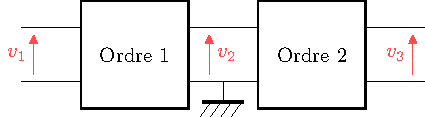
\includegraphics[width=0.6\linewidth]{butterworth_filtre_cascade-plain}
	\end{center}
	Préciser la valeur du facteur de qualité du filtre d'ordre 2.
}{%
	Pour mettre des filtres en cascade et avoir $\Hu = \Hu_1\Hu_2$, il
	faut que l'impédance de sortie du filtre 1 soit faible devant
	l'impédance d'entrée du filtre 2. Dans ce cas, on utilise un filtre
	d'ordre 1 avec un numérateur constant (donc un passe-bas de la forme
	$\Hu_1 = \frac{H_1}{1 + \jx}$), et un filtre
	d'ordre 2 avec un numérateur lui aussi constant~: soit un passe-bas soit
	un passe-bande. Le passe-bande fait intervenir $\jj Q \left( x -
		\frac{1}{x} \right)$ au dénominateur, donc il est plus simple d'utiliser
	une passe-bas d'ordre 2 avec $1 + \jj/Q x + (\jx)^2$ au dénominateur~:
	\begin{gather*}
		\Hu
		= \frac{H_1}{1+ \jx}\times \frac{H_2}{1 + \dfrac{\jj}{Q}x +
			(\jx)^2}
		= \frac{H_1H_2}{1 + \jx \left( 1 + \dfrac{1}{Q} \right)
			+ (\jx)^2 \left( 1 + \dfrac{1}{Q^2} \right) + (\jx)^3}
	\end{gather*}
	Pour trouver un filtre de \textsc{Butterworth} d'ordre 3 de cette
	manière, il faut donc $H_1 = H_2 = 1$ et \fbox{$Q = 1$}.
}

\end{document}
